\documentclass{article}
\usepackage{graphicx}

\begin{document}

\title{Homework Submission Servlet Working Specification}
\author{Mike Burns}
\date{\today}

\maketitle

\section{User Interface}\label{sec:ui}

\begin{figure}[h]
\centering
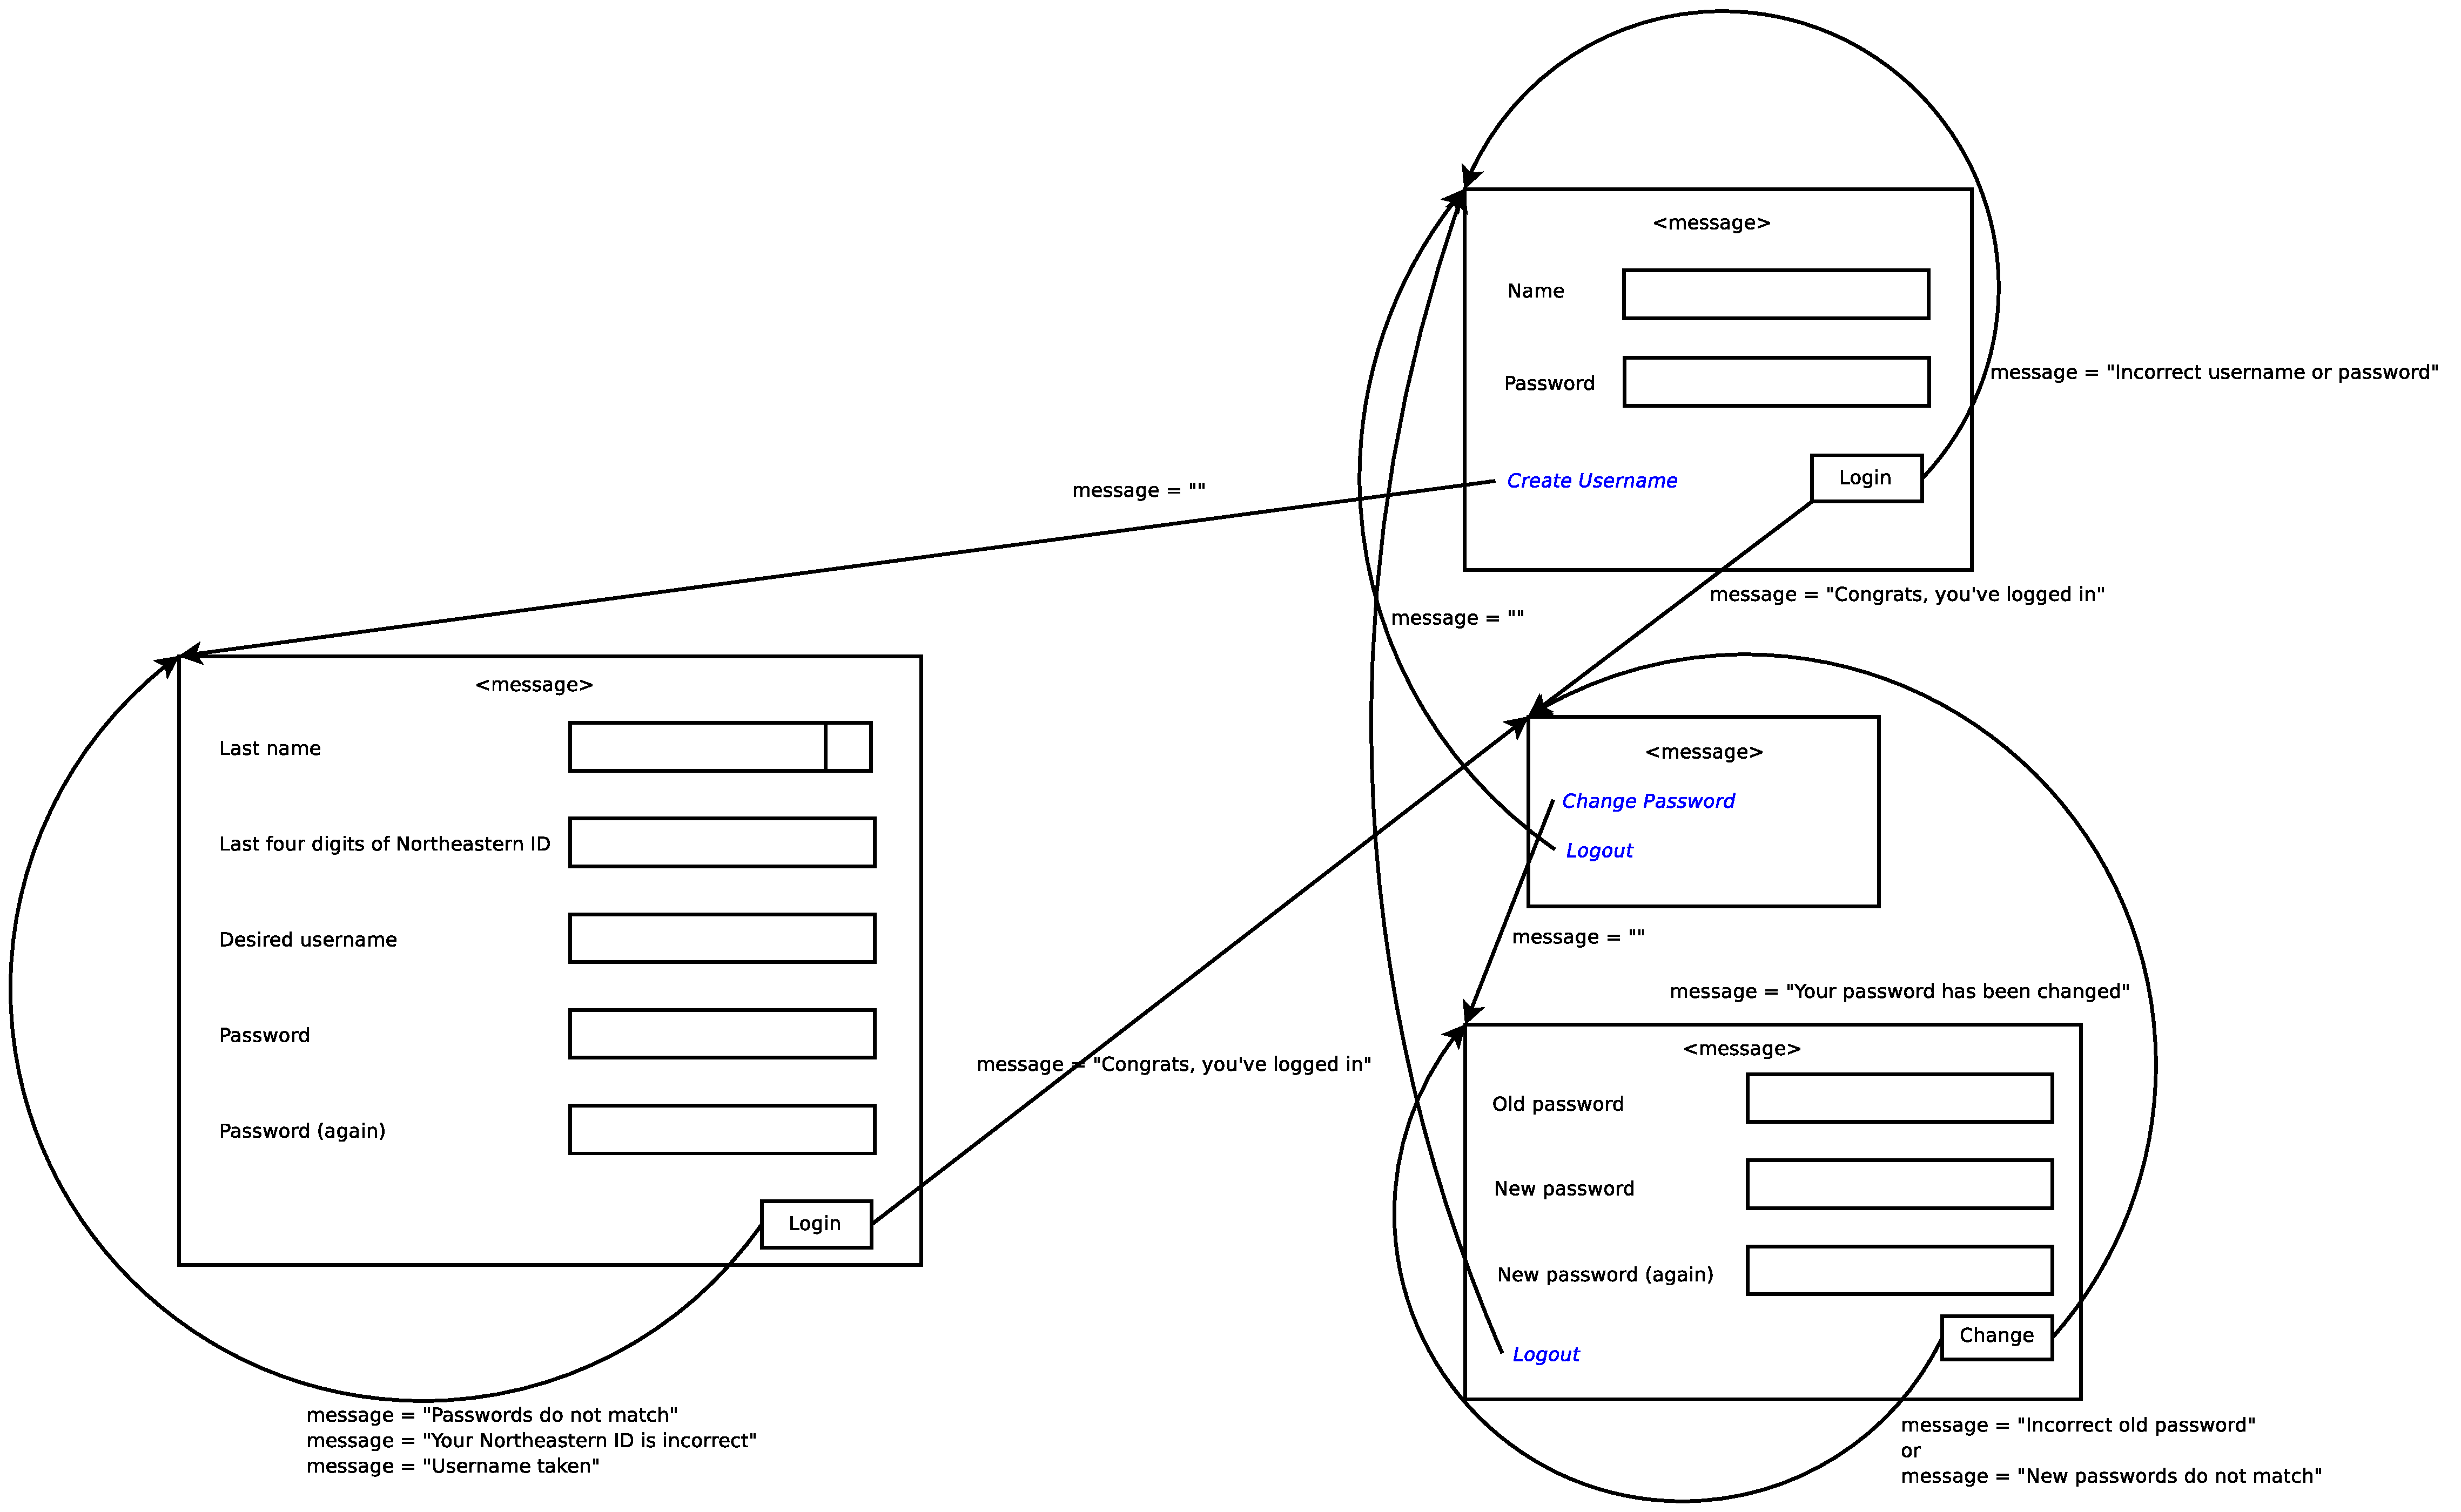
\includegraphics[scale=.35]{servlet.eps}
\caption{The servlet user interface, with interactions}
\label{fig:ui}
\end{figure}

\section{Use Cases}\label{sec:usecases}

\begin{itemize}
\item{A user enters an invalid username and/or password pair.}
\item{A user logs in, then logs out.}
\item{A user logs in, then closes the Web browser.}
\item{A user logs in, logs out, uses the back button once, then logs out again.}
\item{The Web server is restarted by the TA or instructor.}
\item{The password file is editted, with the server stopped, by the TA or
instructor.}
\end{itemize}

\pagebreak

\section{Architecture}\label{sec:arch}

\begin{figure}[h]
\centering
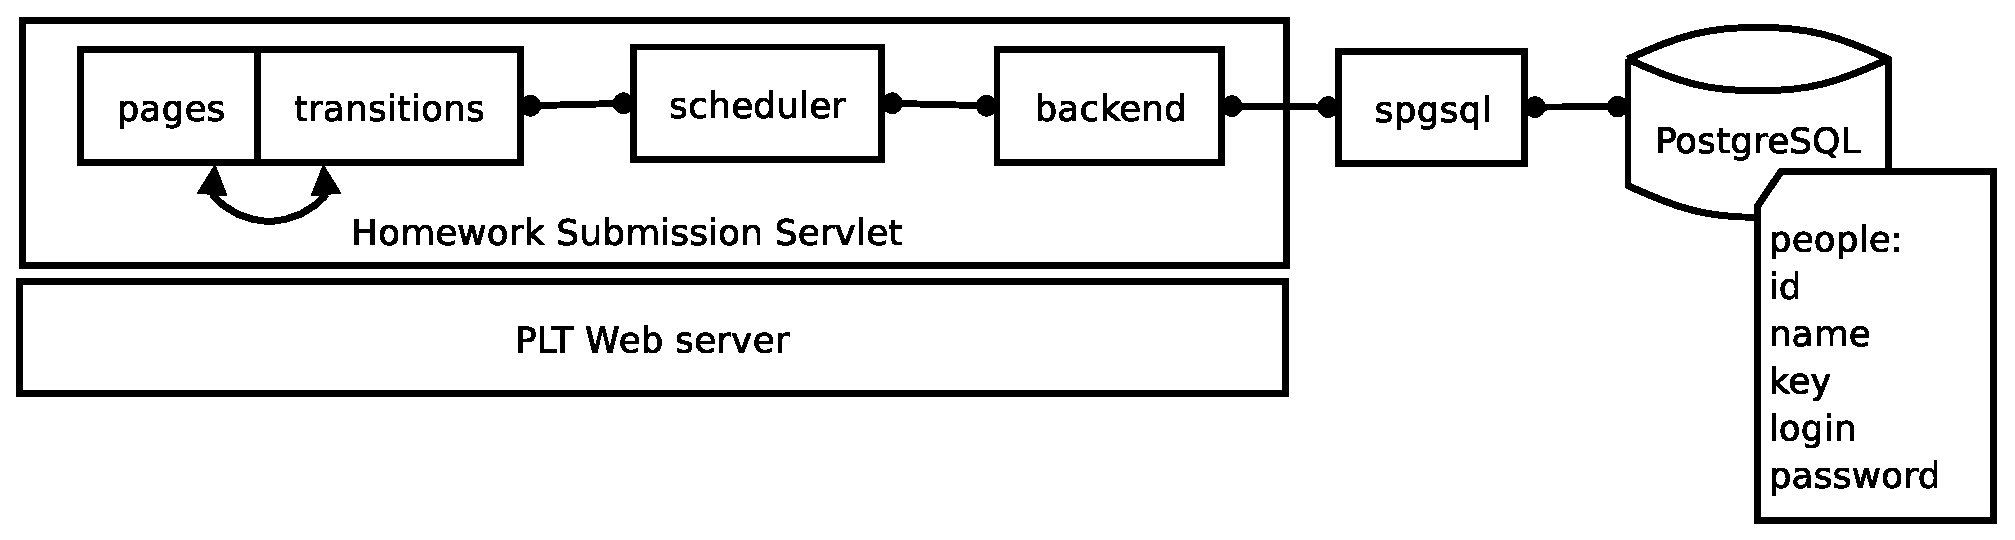
\includegraphics[scale=.35]{architecture.eps}
\caption{The high-level view of the homework submission servlet}
\label{fig:architecture}
\end{figure}

\begin{figure}[h]
\centering
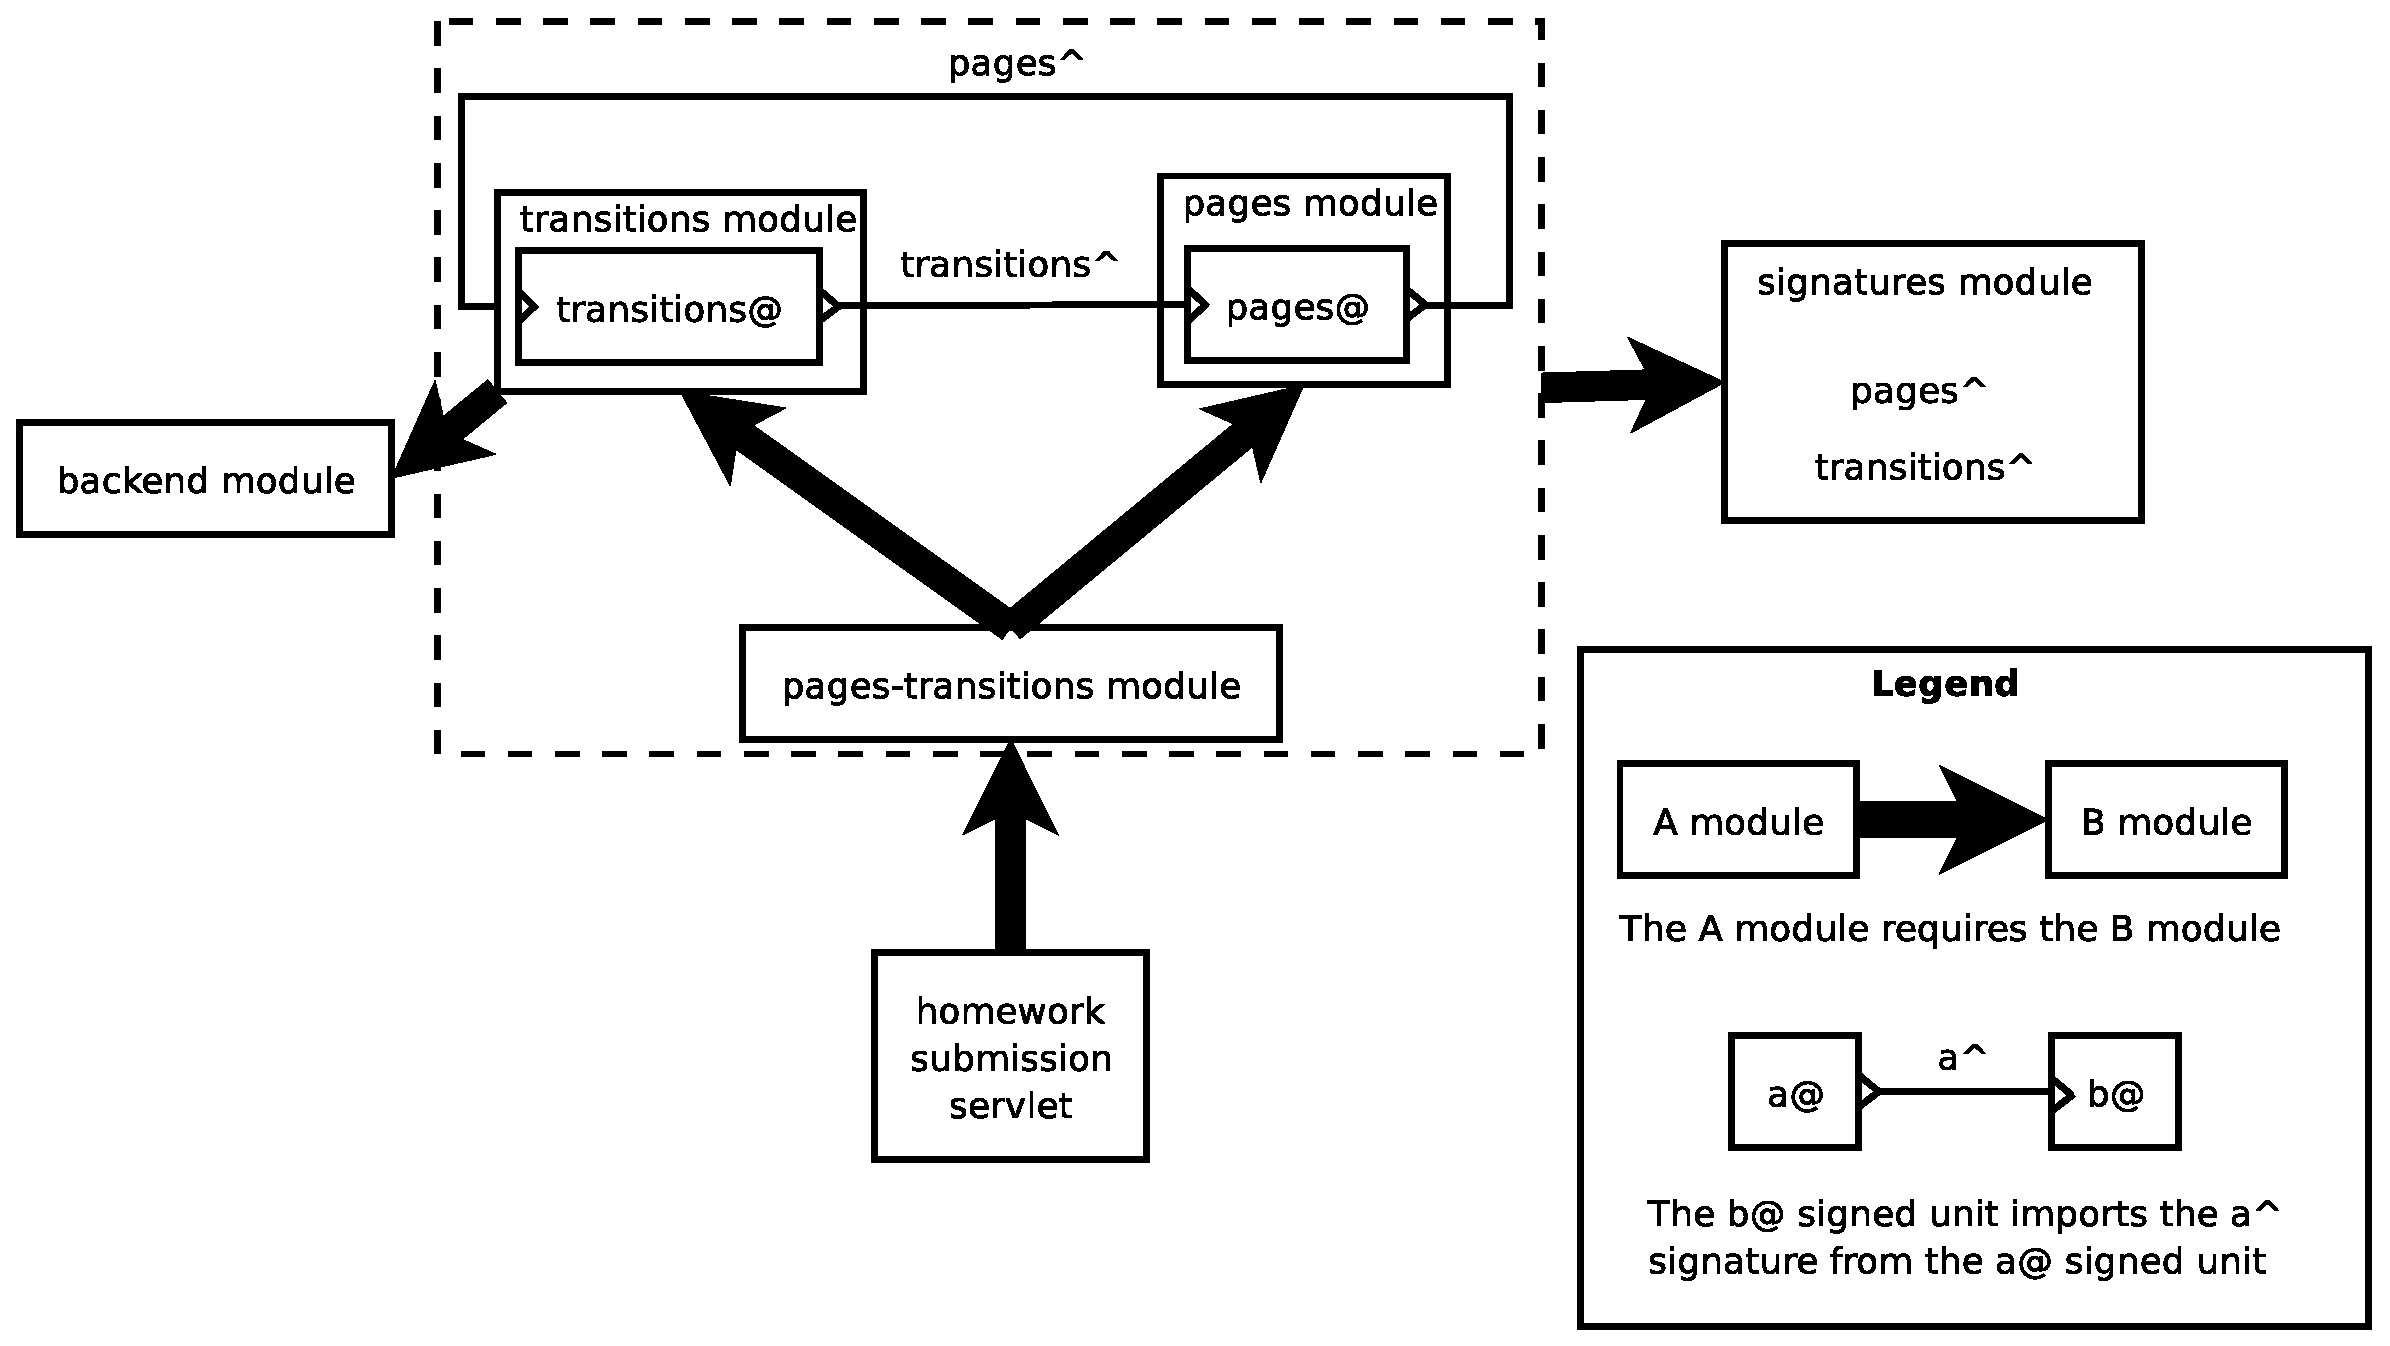
\includegraphics[scale=.35]{design.eps}
\caption{The module and unit layout of the homework submission servlet}
\label{fig:layout}
\end{figure}

The homework submission servlet is driven by the PLT Web server. It is a simple
program that calls the initial transition to send the initial login page to
the client (Web browser).

The module \verb|pages-transitions| invokes and provides all from the signed
units \verb|pages@| and \verb|transitions@|. The functions defined in the
\verb|pages@| signed unit are \verb|xexpr/callback|; that is, they are Web
pages with embedded procedures. These embedded procedures (``transitions'')
have the contract\\
\verb|(request? . -> . (union xexpr? xexpr/callback?))|.

The functions provided from the \verb|pages^| signature are
\begin{itemize}
\item{page-login}
\item{page-logged-in}
\end{itemize}

Pages follow the template:

\begin{verbatim}
(define (page-foo ...)
 `(html (head (title ...))
    (body (h1 ...)
      ...
      (a ((href ,(transition-bar ...))) "Bar")
      ...)))
\end{verbatim}

Transitions are defined in the \verb|transitions@| signed unit. These are the
procedures embedded in the pages, defined in the \verb|pages@| signed unit. The
procedures provided from the \verb|transitions^| signature are
\begin{itemize}
\item{transition-login}
\item{transition-logged-in}
\item{transition-log-out}
\end{itemize}

These procedures have the form:

\begin{verbatim}
(define (transition-foo ...)
  (lambda (req)
    (let* ((a (backend-a)) ...)
      (send/suspend/callback (page-foo a)))))
\end{verbatim}

%The \verb|let*/critical| form treats the bindings of a \verb|let*| as a
%critical block; that is, the bindings are blocked by a semaphore. The body
%of \verb|let*/critical| is outside the critical block. Other available forms
%are \verb|let/critical|, which is like \verb|let*/critical| except it uses
%\verb|let| instead of \verb|let*| semantics; and \verb|critical|, which
%encloses a critical block but binds no variables.

The backend module provides procedures only used by the procedures defined in
the \verb|transitions@| signed unit. These procedures affect the database by
selecting data from, inserting data into, or updating data in the data base.

The data base is a simple file containing a data structure with the contract
\verb|(listof (list/c string? string?))|. The first string is the username, the
second string the MD5-encrypted password. The username must be unique.


\section{Testing}\label{sec:tests}

The simulated server framework uses existing Web server modules to create its
own server, then drives the servlet through this server.

%%% 1. Clean up interface for framework
%%% 2. Document
%%% 3. Replace this will a reference to the documentation from (2).

The following tests must pass, using the simulated server framework:

\begin{itemize}
\item{A user enters an invalid username and/or password.}
\item{A user logs in, then logs out.}
\item{A user logs in, then closes the Web browser.}
\item{A user logs in, logs out, goes back to the logged-in page, and logs out
again.}
%%% Intentionally not tested
%\item{The password file is modified to add a user.}
%\item{The password file is modified to remove a user.}
%\item{The password file is corrupt.}
\end{itemize}

%%% Note yet done. Not sure how best to do this, either.
In addition, the script to start and stop the Web server must work for all TAs
and instructors.

\subsection{Stress Testing}\label{subsec:stresstests}

The stress-test suite drives the servlet using HTTP. This is accomplished with
\verb|get-pure-port| and \verb|call/input-url|, both from the \verb|url.ss|
module in the \verb|net| collection.

\subsubsection{Memory Stress}\label{subsubsec:mem-stress}

These tests will be run in an unbounded loop.

\begin{itemize}
\item{A user logs in, then closes the Web browser.}
\end{itemize}

\subsubsection{Concurrency Tests}\label{subsubsec:parrallel-stress}

These tests will be run in parrallel with themselves, in an unbounded loop.

\begin{itemize}
\item{None yet.}
\end{itemize}

%An hourly automated test will be run against the live servlet; if this test
%fails, an email notification will be sent and the Web server restarted.

\section{Documentation}\label{sec:docs}

The documentation provided with this servlet are this outline and three
documents each describing typical use cases for instructors, teaching
assistants, and students, respecitively.

\end{document}
